% --- IMPORTS ---
\documentclass[leqno]{article}
\usepackage{graphicx}
\usepackage{dsfont}
\usepackage{mathtools}
\usepackage{amssymb}
\usepackage{amsmath}
\usepackage{amsthm}
\usepackage{float}
\usepackage{ragged2e}
\usepackage{tensor}
\usepackage{fancyhdr}
\usepackage{empheq}
\usepackage[most]{tcolorbox}
\usepackage{enumitem}
\usepackage{dirtytalk}
\usepackage{marginnote}
\usepackage{microtype}
\usepackage[
  a4paper,
  left=0.8in,
  right=1in,
  top=1in,
  bottom=0.5in,
  headheight=14pt,
  headsep=0.4in
]{geometry}
\setlength{\parindent}{0cm}
% --- TikZ Packages ---
\usepackage{pgfplots}
\pgfplotsset{compat=1.18}
\usepgfplotslibrary{fillbetween, polar}
\usetikzlibrary{calc, positioning}
\usetikzlibrary{angles, quotes}
\usetikzlibrary{arrows.meta}
\usetikzlibrary{decorations.pathreplacing, decorations.markings}
\usetikzlibrary{patterns}
\usetikzlibrary{intersections}
% --- URL Packages ---
\usepackage[colorlinks=true,linkcolor=red,citecolor=magenta,urlcolor=black]{hyperref}%
\urlstyle{same}
% --- END OF IMPORTS ---

% --- CUSTOM COMMANDS ---
\RenewDocumentCommand{\marks}{o m}{%
  \IfValueTF{#1}%
    {\marginnote{\raggedright\textbf{[#2]}}[#1]}%
    {\marginnote{\raggedright\textbf{[#2]}}}%
}
\newcommand{\vspacerule}[2]{%
  \par\vspace*{#1}%
  \noindent\hrulefill\par
  \vspace*{#2}%
}
\definecolor{scarlet}{RGB}{205, 40, 75}
\newcommand{\questionitem}{%
  \item\phantomsection
  \addcontentsline{toc}{section}{Question \number\value{enumi}}%
}
\renewcommand{\contentsname}{Questions}
% --- END OF CUSTOM COMMANDS ---

% --- HEADER CONFIG ---
\pagestyle{fancy}
\fancyhead{}
\fancyfoot{}
\renewcommand{\headrulewidth}{0.9pt}
\lhead{\textit{Solutions} - Integration by Parts}
\chead{}
\rhead{\href{https://danieljsmith.org}{danieljsmith.org}}
% --- END OF HEADER CONFIG ---

\begin{document}
\vspace*{20pt}
\tableofcontents
\newpage
\begin{enumerate}[
  label=\textbf{\arabic*.},
  leftmargin=*,
  topsep=0pt,
  partopsep=0pt,
  parsep=0pt
]

% ---- Question 1 ----
\questionitem

Given that
\[
y = \arctan\left(\frac{x-2}{x+2}\right)
\]
where $x\ne -2$ \\
\begin{enumerate}[label=\textbf{(\alph*)}]
  \item find $\dfrac{\mathrm{d}y}{\mathrm{d}x}$, giving your answer in its simplest form. \marks{2} \\
  \item Use integration by parts to find
  \[
  \int \arctan\left(\frac{x-2}{x+2}\right)\,\mathrm{d}x
  \]
  \marks[-20pt]{4}
\end{enumerate}

\vspace*{10pt}

\begin{tcolorbox}[colback=white, colframe=scarlet, title={\textbf{Solution}}, breakable, grow to left by=6mm, grow to right by=10mm]
\begin{enumerate}[label=\textbf{(\alph*)}]
  \item Let
\[
u=\frac{x-2}{x+2}
\]
so that
\[
y=\arctan u
\]

Using the chain rule,
\[
\frac{\mathrm{d}y}{\mathrm{d}x}=\frac{1}{1+u^2}\cdot \frac{\mathrm{d}u}{\mathrm{d}x}
\]

Now differentiate $u$:
\begin{align*}
\frac{\mathrm{d}u}{\mathrm{d}x}
&=\frac{(x+2)(1)-(x-2)(1)}{(x+2)^2} \\
&=\frac{x+2-x+2}{(x+2)^2} \\
&=\frac{4}{(x+2)^2}
\end{align*}

Hence
\begin{align*}
\frac{\mathrm{d}y}{\mathrm{d}x}
&=\frac{1}{1+\left(\frac{x-2}{x+2}\right)^2}\cdot \frac{4}{(x+2)^2} \\
&=\frac{4}{(x+2)^2+(x-2)^2} \\
&=\frac{4}{(x^2+4x+4)+(x^2-4x+4)} \\
&=\frac{4}{2x^2+8} \\
&=\frac{2}{x^2+4}
\end{align*}

Therefore,
\[
\frac{\mathrm{d}y}{\mathrm{d}x}=\frac{2}{x^2+4}
\]

  \item Let
\[
I=\int \arctan\left(\frac{x-2}{x+2}\right)\,\mathrm{d}x
\]

Use integration by parts with
\[
u=\arctan\left(\frac{x-2}{x+2}\right),
\qquad
\frac{\mathrm{d}v}{\mathrm{d}x}=1
\]
Then
\[
v=x
\qquad\text{and}\qquad
\frac{\mathrm{d}u}{\mathrm{d}x}=\frac{2}{x^2+4}
\]
from part (a).

Using
\[
\int u\,\frac{\mathrm{d}v}{\mathrm{d}x}\,\mathrm{d}x
=uv-\int v\,\frac{\mathrm{d}u}{\mathrm{d}x}\,\mathrm{d}x
\]
gives
\begin{align*}
I
&=x\arctan\left(\frac{x-2}{x+2}\right)-\int x\cdot \frac{2}{x^2+4}\,\mathrm{d}x \\
&=x\arctan\left(\frac{x-2}{x+2}\right)-\int \frac{2x}{x^2+4}\,\mathrm{d}x
\end{align*}

To evaluate the remaining integral, let
\[
t=x^2+4
\]
so that
\[
\frac{\mathrm{d}t}{\mathrm{d}x}=2x
\qquad\Rightarrow\qquad
\mathrm{d}t=2x\,\mathrm{d}x
\]

Therefore
\begin{align*}
\int \frac{2x}{x^2+4}\,\mathrm{d}x
&=\int \frac{1}{t}\,\mathrm{d}t \\
&=\ln t + C \\
&=\ln(x^2+4)+C
\end{align*}

So
\[
I=x\arctan\left(\frac{x-2}{x+2}\right)-\ln(x^2+4)+C
\]

Hence,
\[
\int \arctan\left(\frac{x-2}{x+2}\right)\,\mathrm{d}x
=
x\arctan\left(\frac{x-2}{x+2}\right)-\ln(x^2+4)+C
\]
\end{enumerate}
\end{tcolorbox}


\newpage

% ---- Question 2 ----
\questionitem
Use integration by parts to find


  \[
  \int_0^2 x^2 \ln(1+x)\,\mathrm{d}x
  \]
  
  giving your answer in the form $a + b\ln 3$, where $a$ and $b$ are constants to be found. \marks{5} \\

\vspace*{10pt}

\begin{tcolorbox}[colback=white, colframe=scarlet, title={\textbf{Solution}}, breakable, grow to left by=6mm, grow to right by=10mm]
Let
\[
I=\int_0^2 x^2\ln(1+x)\,\,\mathrm{d}x
\]

Use integration by parts with
\[
u=\ln(1+x), \qquad \frac{\mathrm{d}v}{\mathrm{d}x}=x^2
\]
so that
\[
\frac{\mathrm{d}u}{\mathrm{d}x}=\frac{1}{1+x}, \qquad v=\frac{x^3}{3}
\]

Then
\begin{align*}
I&=\left[\frac{x^3}{3}\ln(1+x)\right]_0^2-\int_0^2 \frac{x^3}{3(1+x)}\,\,\mathrm{d}x \\
&=\left[\frac{x^3}{3}\ln(1+x)\right]_0^2-\frac13\int_0^2 \frac{x^3}{1+x}\,\,\mathrm{d}x
\end{align*}

Now simplify the fraction:
\[
\frac{x^3}{1+x}=x^2-x+1-\frac{1}{1+x}
\]
since
\[
(1+x)(x^2-x+1)=x^3+1
\]

So
\begin{align*}
\int_0^2 \frac{x^3}{1+x}\,\,\mathrm{d}x
&=\int_0^2 \left(x^2-x+1-\frac{1}{1+x}\right)\mathrm{d}x \\
&=\left[\frac{x^3}{3}-\frac{x^2}{2}+x-\ln(1+x)\right]_0^2 \\
&=\left(\frac{8}{3}-2+2-\ln 3\right)-\left(0-0+0-\ln 1\right) \\
&=\frac{8}{3}-\ln 3
\end{align*}

Also,
\[
\left[\frac{x^3}{3}\ln(1+x)\right]_0^2=\frac{8}{3}\ln 3
\]

Hence
\begin{align*}
I&=\frac{8}{3}\ln 3-\frac13\left(\frac{8}{3}-\ln 3\right) \\
&=\frac{8}{3}\ln 3-\frac{8}{9}+\frac13\ln 3 \\
&=3\ln 3-\frac{8}{9}
\end{align*}

Therefore
\[
\int_0^2 x^2\ln(1+x)\,\,\mathrm{d}x=-\frac89+3\ln 3
\]

So
\[
a=-\frac89, \qquad b=3
\]
\end{tcolorbox}


\newpage

% ---- Question 3 ----
\questionitem

Use integration by parts to find 

\[
\int \operatorname{arsinh}(2x+1)\, \mathrm{d}x
\]

giving your answer in terms of logarithms. \marks{5}

\vspace*{10pt}

\begin{tcolorbox}[colback=white, colframe=scarlet, title={\textbf{Solution}}, breakable, grow to left by=6mm, grow to right by=10mm]
Let
\[
I=\int \operatorname{arsinh}(2x+1)\,\mathrm{d}x
\]

Use the substitution
\[
t=2x+1 \qquad \Rightarrow \qquad \mathrm{d}x=\frac{1}{2}\,\mathrm{d}t
\]

Then
\[
I=\frac{1}{2}\int \operatorname{arsinh}(t)\,\mathrm{d}t
\]

Now integrate by parts. Take
\[
U=\operatorname{arsinh}(t), \qquad \frac{\mathrm{d}V}{\mathrm{d}t}=1
\]
so that
\[
\frac{\mathrm{d}U}{\mathrm{d}t}=\frac{1}{\sqrt{t^2+1}}, \qquad V=t
\]

Using
\[
\int U\,\frac{\mathrm{d}V}{\mathrm{d}t}\,\mathrm{d}t=UV-\int V\,\frac{\mathrm{d}U}{\mathrm{d}t}\,\mathrm{d}t
\]
gives
\begin{align*}
\int \operatorname{arsinh}(t)\,\mathrm{d}t
&= t\operatorname{arsinh}(t)-\int \frac{t}{\sqrt{t^2+1}}\,\mathrm{d}t
\end{align*}

Now
\[
\frac{\mathrm{d}}{\mathrm{d}t}\bigl(\sqrt{t^2+1}\bigr)=\frac{t}{\sqrt{t^2+1}}
\]
so
\[
\int \frac{t}{\sqrt{t^2+1}}\,\mathrm{d}t=\sqrt{t^2+1}
\]

Hence
\[
\int \operatorname{arsinh}(t)\,\mathrm{d}t=t\operatorname{arsinh}(t)-\sqrt{t^2+1}+C
\]

Therefore
\[
I=\frac{1}{2}\left(t\operatorname{arsinh}(t)-\sqrt{t^2+1}\right)+C
\]

Substituting back \(t=2x+1\),
\[
I=\frac{1}{2}\left((2x+1)\operatorname{arsinh}(2x+1)-\sqrt{(2x+1)^2+1}\right)+C
\]

Finally, using
\[
\operatorname{arsinh}(y)=\ln\!\left(y+\sqrt{y^2+1}\right)
\]
we get
\[
\int \operatorname{arsinh}(2x+1)\,\mathrm{d}x
=
\frac{1}{2}\left((2x+1)\ln\!\left(2x+1+\sqrt{(2x+1)^2+1}\right)-\sqrt{(2x+1)^2+1}\right)+C
\]

So the answer in logarithmic form is
\[
\frac{1}{2}\left((2x+1)\ln\!\left(2x+1+\sqrt{(2x+1)^2+1}\right)-\sqrt{(2x+1)^2+1}\right)+C
\]
\end{tcolorbox}


\newpage

% ---- Question 4 ----
\questionitem

\[
h(\theta)=(3\sin\theta-\cos\theta)(\sin\theta+2\cos\theta)
\] \\
\begin{enumerate}[label=\textbf{(\alph*)}]
  \item Show that $h(\theta)=\dfrac{1}{2}-\dfrac{5}{2}\cos 2\theta+\dfrac{5}{2}\sin 2\theta$. \marks{4} \\
  \item Hence, using calculus, find the exact value of
  \[
  \int_{0}^{\frac{\pi}{2}} \left(\frac{\pi}{2}-\theta\right) h(\theta)\,\mathrm{d}\theta
  \]
  \marks[-30pt]{7}
\end{enumerate}

\vspace*{10pt}

\begin{tcolorbox}[colback=white, colframe=scarlet, title={\textbf{Solution}}, breakable, grow to left by=6mm, grow to right by=10mm]
\begin{enumerate}[label=\textbf{(\alph*)}]
\item Expanding the brackets,
\begin{align*}
h(\theta)
&=(3\sin\theta-\cos\theta)(\sin\theta+2\cos\theta)\\
&=3\sin^2\theta+6\sin\theta\cos\theta-\sin\theta\cos\theta-2\cos^2\theta\\
&=3\sin^2\theta+5\sin\theta\cos\theta-2\cos^2\theta
\end{align*}

Now use the double-angle identities
\[
\sin^2\theta=\frac{1-\cos2\theta}{2},\qquad
\cos^2\theta=\frac{1+\cos2\theta}{2},\qquad
\sin\theta\cos\theta=\frac12\sin2\theta
\]

Substituting,
\begin{align*}
h(\theta)
&=3\left(\frac{1-\cos2\theta}{2}\right)+5\left(\frac12\sin2\theta\right)-2\left(\frac{1+\cos2\theta}{2}\right)\\
&=\frac32-\frac32\cos2\theta+\frac52\sin2\theta-1-\cos2\theta\\
&=\frac12-\frac52\cos2\theta+\frac52\sin2\theta
\end{align*}

Hence,
\[
h(\theta)=\frac12-\frac52\cos2\theta+\frac52\sin2\theta
\]

\item Let
\[
I=\int_{0}^{\frac{\pi}{2}}\left(\frac{\pi}{2}-\theta\right)h(\theta)\,\mathrm{d}\theta
\]

Using part (a),
\begin{align*}
I
&=\int_{0}^{\frac{\pi}{2}}\left(\frac{\pi}{2}-\theta\right)\left(\frac12-\frac52\cos2\theta+\frac52\sin2\theta\right)\,\mathrm{d}\theta\\
&=\frac12\int_{0}^{\frac{\pi}{2}}\left(\frac{\pi}{2}-\theta\right)\,\mathrm{d}\theta
-\frac52\int_{0}^{\frac{\pi}{2}}\left(\frac{\pi}{2}-\theta\right)\cos2\theta\,\mathrm{d}\theta
+\frac52\int_{0}^{\frac{\pi}{2}}\left(\frac{\pi}{2}-\theta\right)\sin2\theta\,\mathrm{d}\theta
\end{align*}

We evaluate the three integrals separately.

First,
\begin{align*}
\int_{0}^{\frac{\pi}{2}}\left(\frac{\pi}{2}-\theta\right)\,\mathrm{d}\theta
&=\left[\frac{\pi\theta}{2}-\frac{\theta^2}{2}\right]_{0}^{\frac{\pi}{2}}\\
&=\frac{\pi^2}{4}-\frac{\pi^2}{8}\\
&=\frac{\pi^2}{8}
\end{align*}

So the first term contributes
\[
\frac12\cdot\frac{\pi^2}{8}=\frac{\pi^2}{16}
\]

Now let
\[
B=\int_{0}^{\frac{\pi}{2}}\left(\frac{\pi}{2}-\theta\right)\cos2\theta\,\mathrm{d}\theta
\]

Integrating by parts with
\[
u=\frac{\pi}{2}-\theta,\qquad \frac{\mathrm{d}v}{\mathrm{d}\theta}=\cos2\theta
\]
gives
\[
\frac{\mathrm{d}u}{\mathrm{d}\theta}=-1,\qquad v=\frac12\sin2\theta
\]

Hence,
\begin{align*}
B
&=\left(\frac{\pi}{2}-\theta\right)\left(\frac12\sin2\theta\right)\Bigg|_{0}^{\frac{\pi}{2}}
+\frac12\int_{0}^{\frac{\pi}{2}}\sin2\theta\,\mathrm{d}\theta\\
&=0+\frac12\left[-\frac12\cos2\theta\right]_{0}^{\frac{\pi}{2}}\\
&=\frac12\left(-\frac12\cos\pi+\frac12\cos0\right)\\
&=\frac12\left(\frac12+\frac12\right)\\
&=\frac12
\end{align*}

Next let
\[
C=\int_{0}^{\frac{\pi}{2}}\left(\frac{\pi}{2}-\theta\right)\sin2\theta\,\mathrm{d}\theta
\]

Again integrating by parts with
\[
u=\frac{\pi}{2}-\theta,\qquad \frac{\mathrm{d}v}{\mathrm{d}\theta}=\sin2\theta
\]
gives
\[
\frac{\mathrm{d}u}{\mathrm{d}\theta}=-1,\qquad v=-\frac12\cos2\theta
\]

So,
\begin{align*}
C
&=-\left(\frac{\pi}{2}-\theta\right)\left(\frac12\cos2\theta\right)\Bigg|_{0}^{\frac{\pi}{2}}
-\frac12\int_{0}^{\frac{\pi}{2}}\cos2\theta\,\mathrm{d}\theta\\
&=-\left[ \left(\frac{\pi}{2}-\theta\right)\frac12\cos2\theta \right]_{0}^{\frac{\pi}{2}}
-\frac12\left[\frac12\sin2\theta\right]_{0}^{\frac{\pi}{2}}\\
&=\frac{\pi}{4}-0\\
&=\frac{\pi}{4}
\end{align*}

Substituting these into the expression for \(I\),
\begin{align*}
I
&=\frac{\pi^2}{16}-\frac52\left(\frac12\right)+\frac52\left(\frac{\pi}{4}\right)\\
&=\frac{\pi^2}{16}-\frac54+\frac{5\pi}{8}\\
&=\frac{\pi^2+10\pi-20}{16}
\end{align*}

Therefore, the exact value is
\[
\int_{0}^{\frac{\pi}{2}}\left(\frac{\pi}{2}-\theta\right)h(\theta)\,\mathrm{d}\theta
=\frac{\pi^2+10\pi-20}{16}
\]

This is approximately \(1.33\).
\end{enumerate}
\end{tcolorbox}


\newpage

% ---- Question 5 ----
\questionitem

\begin{enumerate}[label=\textbf{(\alph*)}]
  \item Find
  \[
  \int x^2\arctan x\,\mathrm{d}x
  \]
  \marks[-20pt]{5}
  \item Hence find the exact value of
  \[
  \int_0^1 x^2\arctan x\,\mathrm{d}x
  \]
  \marks[-20pt]{2}
\end{enumerate}

\vspace*{10pt}

\begin{tcolorbox}[colback=white, colframe=scarlet, title={\textbf{Solution}}, breakable, grow to left by=6mm, grow to right by=10mm]
\begin{enumerate}[label=\textbf{(\alph*)}]
  \item Let
\[
I=\int x^2\arctan x\,\mathrm{d}x
\]

Use integration by parts with
\[
u=\arctan x,\qquad \frac{\mathrm{d}v}{\mathrm{d}x}=x^2
\]
so that
\[
\frac{\mathrm{d}u}{\mathrm{d}x}=\frac{1}{1+x^2},\qquad v=\frac{x^3}{3}
\]

Then
\begin{align*}
I&=uv-\int v\frac{\mathrm{d}u}{\mathrm{d}x}\,\mathrm{d}x\\
&=\frac{x^3}{3}\arctan x-\int \frac{x^3}{3(1+x^2)}\,\mathrm{d}x\\
&=\frac{x^3}{3}\arctan x-\frac13\int \frac{x^3}{1+x^2}\,\mathrm{d}x
\end{align*}

Now simplify the fraction:
\begin{align*}
\frac{x^3}{1+x^2}
&=x-\frac{x}{1+x^2}
\end{align*}
since
\[
x-\frac{x}{1+x^2}=\frac{x(1+x^2)-x}{1+x^2}=\frac{x^3}{1+x^2}
\]

So
\begin{align*}
I&=\frac{x^3}{3}\arctan x-\frac13\int\left(x-\frac{x}{1+x^2}\right)\,\mathrm{d}x\\
&=\frac{x^3}{3}\arctan x-\frac13\left(\int x\,\mathrm{d}x-\int \frac{x}{1+x^2}\,\mathrm{d}x\right)
\end{align*}

Now
\[
\int x\,\mathrm{d}x=\frac{x^2}{2}
\]
and, using the substitution $1+x^2$,
\[
\int \frac{x}{1+x^2}\,\mathrm{d}x=\frac12\ln(1+x^2)
\]

Hence
\begin{align*}
I&=\frac{x^3}{3}\arctan x-\frac13\left(\frac{x^2}{2}-\frac12\ln(1+x^2)\right)+C\\
&=\frac{x^3}{3}\arctan x-\frac{x^2}{6}+\frac16\ln(1+x^2)+C
\end{align*}

Therefore,
\[
\int x^2\arctan x\,\mathrm{d}x=\frac{x^3}{3}\arctan x-\frac{x^2}{6}+\frac16\ln(1+x^2)+C
\]

  \item Using the result from part (a),
\[
\int_0^1 x^2\arctan x\,\mathrm{d}x
=
\left[\frac{x^3}{3}\arctan x-\frac{x^2}{6}+\frac16\ln(1+x^2)\right]_0^1
\]

Substituting the limits:
\begin{align*}
\int_0^1 x^2\arctan x\,\mathrm{d}x
&=\left(\frac13\arctan1-\frac16+\frac16\ln 2\right)-\left(0-0+\frac16\ln 1\right)\\
&=\frac13\cdot\frac{\pi}{4}-\frac16+\frac16\ln 2
\end{align*}

Since $\ln 1=0$,
\[
\int_0^1 x^2\arctan x\,\mathrm{d}x=\frac{\pi}{12}-\frac16+\frac{\ln 2}{6}
\]

So the exact value is
\[
\frac{\pi+2\ln 2-2}{12}
\]
\end{enumerate}
\end{tcolorbox}


\newpage

% ---- Question 6 ----
\questionitem

\begin{enumerate}[label=\textbf{(\roman*)}]
  \item Sketch the graph of $y=\arctan x$ for $x\in\mathbb{R}$, indicating any horizontal asymptotes. \marks{1} \\
  \item Prove that
  \[
  \frac{\mathrm{d}}{\mathrm{d}x}(\arctan x)=\frac{1}{1+x^2}
  \]
  \marks[-20pt]{4}
  \item Using integration by parts and suitable substitutions, show that
  \[
  \int_0^1 x(\arctan x)^2\,\mathrm{d}x=\frac{\pi^2}{16}-\frac{\pi}{4}+\frac{1}{2}\ln 2
  \]
  \marks[-30pt]{6}
\end{enumerate}

\vspace*{10pt}

\begin{tcolorbox}[colback=white, colframe=scarlet, title={\textbf{Solution}}, breakable, grow to left by=6mm, grow to right by=10mm]
\begin{enumerate}[label=\textbf{(\roman*)}]
  \item The graph of \(y=\arctan x\) is an increasing odd curve passing through \((0,0)\).

As \(x\to\infty\), \(y\to \dfrac{\pi}{2}\), and as \(x\to -\infty\), \(y\to -\dfrac{\pi}{2}\).

So the horizontal asymptotes are
\[
y=\frac{\pi}{2}
\qquad \text{and} \qquad
y=-\frac{\pi}{2}
\]

\begin{center}
\begin{tikzpicture}
\begin{axis}[
width=8cm,
height=5cm,
axis lines=middle,
xmin=-5, xmax=5,
ymin=-2, ymax=2,
xlabel={$x$},
ylabel={$y$},
xtick={0},
ytick={-1.5708,0,1.5708},
yticklabels={$-\frac{\pi}{2}$,$0$,$\frac{\pi}{2}$},
samples=200
]
\addplot[domain=-5:5] {atan(x)*pi/180};
\addplot[dashed] coordinates {(-5,1.5708) (5,1.5708)};
\addplot[dashed] coordinates {(-5,-1.5708) (5,-1.5708)};
\end{axis}
\end{tikzpicture}
\end{center}

  \item Let
\[
y=\arctan x
\]
Then
\[
x=\tan y
\]

Differentiate implicitly with respect to \(x\):
\[
1=\sec^2 y\,\frac{\mathrm{d}y}{\mathrm{d}x}
\]

So
\begin{align*}
\frac{\mathrm{d}y}{\mathrm{d}x}
&=\frac{1}{\sec^2 y}\\
&=\frac{1}{1+\tan^2 y}\\
&=\frac{1}{1+x^2}
\end{align*}

since \(\tan y=x\).

Therefore
\[
\frac{\mathrm{d}}{\mathrm{d}x}(\arctan x)=\frac{1}{1+x^2}
\]

  \item Let
\[
I=\int_0^1 x(\arctan x)^2\,\mathrm{d}x
\]

Use integration by parts with
\[
u=(\arctan x)^2,
\qquad
\frac{\mathrm{d}v}{\mathrm{d}x}=x
\]
Then
\[
\frac{\mathrm{d}u}{\mathrm{d}x}=2(\arctan x)\cdot \frac{1}{1+x^2},
\qquad
v=\frac{x^2}{2}
\]

Hence
\begin{align*}
I
&=\left[\frac{x^2}{2}(\arctan x)^2\right]_0^1-\int_0^1 \frac{x^2}{2}\cdot 2\frac{\arctan x}{1+x^2}\,\mathrm{d}x\\
&=\left[\frac{x^2}{2}(\arctan x)^2\right]_0^1-\int_0^1 \frac{x^2\arctan x}{1+x^2}\,\mathrm{d}x\\
&=\frac{1}{2}\left(\frac{\pi}{4}\right)^2-\int_0^1 \frac{x^2\arctan x}{1+x^2}\,\mathrm{d}x\\
&=\frac{\pi^2}{32}-\int_0^1 \frac{x^2\arctan x}{1+x^2}\,\mathrm{d}x
\end{align*}

Now
\[
\frac{x^2}{1+x^2}=1-\frac{1}{1+x^2}
\]
so
\begin{align*}
I
&=\frac{\pi^2}{32}-\int_0^1 \arctan x\,\mathrm{d}x+\int_0^1 \frac{\arctan x}{1+x^2}\,\mathrm{d}x
\end{align*}

We now evaluate these two integrals separately.

First, let
\[
J=\int_0^1 \arctan x\,\mathrm{d}x
\]
Using integration by parts with
\[
u=\arctan x,
\qquad
\frac{\mathrm{d}v}{\mathrm{d}x}=1
\]
gives
\[
\frac{\mathrm{d}u}{\mathrm{d}x}=\frac{1}{1+x^2},
\qquad
v=x
\]
So
\begin{align*}
J
&=\left[x\arctan x\right]_0^1-\int_0^1 \frac{x}{1+x^2}\,\mathrm{d}x\\
&=\frac{\pi}{4}-\int_0^1 \frac{x}{1+x^2}\,\mathrm{d}x
\end{align*}

Now use the substitution \(t=1+x^2\), so \(\mathrm{d}t=2x\,\mathrm{d}x\). Then
\begin{align*}
\int_0^1 \frac{x}{1+x^2}\,\mathrm{d}x
&=\frac{1}{2}\int_1^2 \frac{1}{t}\,\mathrm{d}t\\
&=\frac{1}{2}\left[\ln t\right]_1^2\\
&=\frac{1}{2}\ln 2
\end{align*}

Therefore
\[
J=\frac{\pi}{4}-\frac{1}{2}\ln 2
\]

Next, let
\[
K=\int_0^1 \frac{\arctan x}{1+x^2}\,\mathrm{d}x
\]
Use the substitution
\[
t=\arctan x
\]
Then
\[
x=\tan t,
\qquad
\mathrm{d}x=\sec^2 t\,\mathrm{d}t,
\qquad
1+x^2=1+\tan^2 t=\sec^2 t
\]
When \(x=0\), \(t=0\), and when \(x=1\), \(t=\dfrac{\pi}{4}\). Hence
\begin{align*}
K
&=\int_0^{\pi/4} \frac{t}{\sec^2 t}\sec^2 t\,\mathrm{d}t\\
&=\int_0^{\pi/4} t\,\mathrm{d}t\\
&=\left[\frac{t^2}{2}\right]_0^{\pi/4}\\
&=\frac{\pi^2}{32}
\end{align*}

Substitute \(J\) and \(K\) back into the expression for \(I\):
\begin{align*}
I
&=\frac{\pi^2}{32}-\left(\frac{\pi}{4}-\frac{1}{2}\ln 2\right)+\frac{\pi^2}{32}\\
&=\frac{\pi^2}{16}-\frac{\pi}{4}+\frac{1}{2}\ln 2
\end{align*}

Therefore
\[
\int_0^1 x(\arctan x)^2\,\mathrm{d}x
=
\frac{\pi^2}{16}-\frac{\pi}{4}+\frac{1}{2}\ln 2
\]
\end{enumerate}
\end{tcolorbox}


\newpage

% ---- Question 7 ----
\questionitem

\begin{enumerate}[label=\textbf{(\alph*)}]
  \item Find
  \[
  \int x^3\arctan x\,\mathrm{d}x
  \]
  \marks[-20pt]{5}
  \item Hence find the exact value of
  \[
  \int_0^{\sqrt{3}} x^3\arctan x\,\mathrm{d}x
  \]
  \marks[-20pt]{2}
\end{enumerate}

\vspace*{10pt}

\begin{tcolorbox}[colback=white, colframe=scarlet, title={\textbf{Solution}}, breakable, grow to left by=6mm, grow to right by=10mm]
\begin{enumerate}[label=\textbf{(\alph*)}]
  \item Use integration by parts with
  \[
  u=\arctan x \qquad \frac{\mathrm{d}v}{\mathrm{d}x}=x^3
  \]
  so that
  \[
  \frac{\mathrm{d}u}{\mathrm{d}x}=\frac{1}{1+x^2}, \qquad v=\frac{x^4}{4}
  \]

  Then
  \begin{align*}
  \int x^3\arctan x\,\mathrm{d}x
  &= \int u\,\frac{\mathrm{d}v}{\mathrm{d}x}\,\mathrm{d}x \\
  &= uv-\int v\,\frac{\mathrm{d}u}{\mathrm{d}x}\,\mathrm{d}x \\
  &= \frac{x^4}{4}\arctan x-\int \frac{x^4}{4(1+x^2)}\,\mathrm{d}x \\
  &= \frac{x^4}{4}\arctan x-\frac14\int \frac{x^4}{1+x^2}\,\mathrm{d}x
  \end{align*}

  Now simplify the fraction by division:
  \[
  \frac{x^4}{1+x^2}=x^2-1+\frac{1}{1+x^2}
  \]
  since
  \[
  (1+x^2)(x^2-1)+1=x^4-1+1=x^4
  \]

  So
  \begin{align*}
  \int x^3\arctan x\,\mathrm{d}x
  &= \frac{x^4}{4}\arctan x-\frac14\int \left(x^2-1+\frac{1}{1+x^2}\right)\,\mathrm{d}x \\
  &= \frac{x^4}{4}\arctan x-\frac14\left(\int x^2\,\mathrm{d}x-\int 1\,\mathrm{d}x+\int \frac{1}{1+x^2}\,\mathrm{d}x\right) \\
  &= \frac{x^4}{4}\arctan x-\frac14\left(\frac{x^3}{3}-x+\arctan x\right)+C \\
  &= \frac{x^4}{4}\arctan x-\frac{x^3}{12}+\frac{x}{4}-\frac14\arctan x+C \\
  &= \frac{x^4-1}{4}\arctan x-\frac{x^3}{12}+\frac{x}{4}+C
  \end{align*}

  Therefore,
  \[
  \int x^3\arctan x\,\mathrm{d}x=\frac{x^4-1}{4}\arctan x-\frac{x^3}{12}+\frac{x}{4}+C
  \]

  \item Using the result from part (a), let
  \[
  F(x)=\frac{x^4-1}{4}\arctan x-\frac{x^3}{12}+\frac{x}{4}
  \]

  Then
  \[
  \int_0^{\sqrt3} x^3\arctan x\,\mathrm{d}x=F(\sqrt3)-F(0)
  \]

  First, at \(x=\sqrt3\),
  \[
  \arctan(\sqrt3)=\frac{\pi}{3}, \qquad (\sqrt3)^4=9, \qquad (\sqrt3)^3=3\sqrt3
  \]
  so
  \begin{align*}
  F(\sqrt3)
  &= \frac{9-1}{4}\cdot \frac{\pi}{3}-\frac{3\sqrt3}{12}+\frac{\sqrt3}{4} \\
  &= \frac{8}{4}\cdot \frac{\pi}{3}-\frac{\sqrt3}{4}+\frac{\sqrt3}{4} \\
  &= \frac{2\pi}{3}
  \end{align*}

  Also,
  \[
  F(0)=\frac{0-1}{4}\arctan 0-0+0=0
  \]

  Hence
  \[
  \int_0^{\sqrt3} x^3\arctan x\,\mathrm{d}x=\frac{2\pi}{3}
  \]

  So the exact value is \(\displaystyle \frac{2\pi}{3}\).
\end{enumerate}
\end{tcolorbox}


\newpage

% ---- Question 8 ----
\questionitem

\begin{enumerate}[label=\textbf{(\alph*)}]
  \item Using the logarithmic form
  \[
  \operatorname{artanh} x = \frac{1}{2}\ln\left(\frac{1+x}{1-x}\right),\qquad |x|<1
  \]
  prove that the derivative of $\operatorname{artanh} x$ is
  \[
  \frac{1}{1-x^2}
  \]
  \marks{5} \\
  \item Hence find
  \[
  \int_0^{1/3} \operatorname{artanh}(2x)\,\mathrm{d}x
  \]
  giving your answer in exact logarithmic form. \marks{5} \\
  \item Noah tries to evaluate
  \[
  \int_0^{1/2} \operatorname{artanh}(2x)\,\mathrm{d}x
  \]
  using his calculator, and gets an error. Explain why. \marks{1} \\
\end{enumerate}

\vspace*{10pt}

\begin{tcolorbox}[colback=white, colframe=scarlet, title={\textbf{Solution}}, breakable, grow to left by=6mm, grow to right by=10mm]
\begin{enumerate}[label=\textbf{(\alph*)}]
  \item Using the given logarithmic form,
\[
\operatorname{artanh}x=\frac12\ln\left(\frac{1+x}{1-x}\right)
=\frac12\bigl[\ln(1+x)-\ln(1-x)\bigr]
\]
for \(|x|<1\).

Differentiate term by term:
\begin{align*}
\frac{\mathrm{d}}{\mathrm{d}x}\bigl(\operatorname{artanh}x\bigr)
&=\frac12\left(\frac{\mathrm{d}}{\mathrm{d}x}\ln(1+x)-\frac{\mathrm{d}}{\mathrm{d}x}\ln(1-x)\right)\\
&=\frac12\left(\frac{1}{1+x}-\frac{-1}{1-x}\right)\\
&=\frac12\left(\frac{1}{1+x}+\frac{1}{1-x}\right)\\
&=\frac12\left(\frac{(1-x)+(1+x)}{(1+x)(1-x)}\right)\\
&=\frac12\left(\frac{2}{1-x^2}\right)\\
&=\frac{1}{1-x^2}
\end{align*}
Hence
\[
\frac{\mathrm{d}}{\mathrm{d}x}\bigl(\operatorname{artanh}x\bigr)=\frac{1}{1-x^2}
\]

  \item On \(0\le x\le \frac13\), we have \(0\le 2x\le \frac23<1\), so \(\operatorname{artanh}(2x)\) is defined.

Let
\[
I=\int_0^{1/3}\operatorname{artanh}(2x)\,\mathrm{d}x
\]
Use integration by parts with
\[
u=\operatorname{artanh}(2x),\qquad \frac{\mathrm{d}v}{\mathrm{d}x}=1
\]
Then
\[
v=x
\]
and from part (a), using the chain rule,
\[
\frac{\mathrm{d}u}{\mathrm{d}x}=\frac{2}{1-(2x)^2}=\frac{2}{1-4x^2}
\]
So
\begin{align*}
I&=\left[x\operatorname{artanh}(2x)\right]_0^{1/3}-\int_0^{1/3}x\cdot \frac{2}{1-4x^2}\,\mathrm{d}x\\
&=\left[x\operatorname{artanh}(2x)\right]_0^{1/3}-\int_0^{1/3}\frac{2x}{1-4x^2}\,\mathrm{d}x
\end{align*}
For the remaining integral, let
\[
t=1-4x^2
\]
Then
\[
\mathrm{d}t=-8x\,\mathrm{d}x
\]
so
\[
2x\,\mathrm{d}x=-\frac14\,\mathrm{d}t
\]
When \(x=0\), \(t=1\), and when \(x=\frac13\), \(t=\frac59\). Therefore
\begin{align*}
\int_0^{1/3}\frac{2x}{1-4x^2}\,\mathrm{d}x
&=-\frac14\int_1^{5/9}\frac{1}{t}\,\mathrm{d}t\\
&=-\frac14\left[\ln t\right]_1^{5/9}\\
&=-\frac14\ln\left(\frac59\right)
\end{align*}
Hence
\begin{align*}
I&=\left[x\operatorname{artanh}(2x)\right]_0^{1/3}+\frac14\ln\left(\frac59\right)\\
&=\frac13\operatorname{artanh}\left(\frac23\right)+\frac14\ln\left(\frac59\right)
\end{align*}
Now use the logarithmic form again:
\begin{align*}
\operatorname{artanh}\left(\frac23\right)
&=\frac12\ln\left(\frac{1+\frac23}{1-\frac23}\right)\\
&=\frac12\ln\left(\frac{5/3}{1/3}\right)\\
&=\frac12\ln 5
\end{align*}
So
\begin{align*}
I&=\frac13\cdot\frac12\ln 5+\frac14\ln\left(\frac59\right)\\
&=\frac16\ln 5+\frac14(\ln 5-\ln 9)\\
&=\frac16\ln 5+\frac14\ln 5-\frac12\ln 3\\
&=\frac{5}{12}\ln 5-\frac12\ln 3
\end{align*}
This can also be written as
\begin{align*}
I&=\frac1{12}\bigl(5\ln 5-6\ln 3\bigr)\\
&=\frac1{12}\ln\left(\frac{5^5}{3^6}\right)\\
&=\frac1{12}\ln\left(\frac{3125}{729}\right)
\end{align*}
Therefore
\[
\int_0^{1/3}\operatorname{artanh}(2x)\,\mathrm{d}x
=\frac{5}{12}\ln 5-\frac12\ln 3
=\frac1{12}\ln\left(\frac{3125}{729}\right)
\]

  \item At the upper limit \(x=\frac12\), we have \(2x=1\), and \(\operatorname{artanh}(1)\) is undefined because \(\operatorname{artanh}t\) is only defined for \(|t|<1\).

So the integrand is not defined at the endpoint, and a calculator treating this as an ordinary definite integral gives an error.
\end{enumerate}
\end{tcolorbox}


\newpage

% ---- Question 9 ----
\questionitem

For $0<x<1$, use integration by parts to find
\[
\int x\,\operatorname{artanh}(2x-1)\,\mathrm{d}x
\]
giving your final answer in terms of logarithms. \marks{6}

\vspace*{10pt}

\begin{tcolorbox}[colback=white, colframe=scarlet, title={\textbf{Solution}}, breakable, grow to left by=6mm, grow to right by=10mm]
Let
\[
I=\int x\,\operatorname{artanh}(2x-1)\,\mathrm{d}x
\]

Use integration by parts with
\[
u=\operatorname{artanh}(2x-1), \qquad \frac{\mathrm{d}v}{\mathrm{d}x}=x
\]
Then
\[
v=\frac{x^2}{2}
\]
and
\begin{align*}
\frac{\mathrm{d}u}{\mathrm{d}x}
&=\frac{2}{1-(2x-1)^2} \\
&=\frac{2}{1-(4x^2-4x+1)} \\
&=\frac{2}{4x-4x^2} \\
&=\frac{1}{2x(1-x)}
\end{align*}

So, by integration by parts,
\begin{align*}
I
&=uv-\int v\,\frac{\mathrm{d}u}{\mathrm{d}x}\,\mathrm{d}x \\
&=\frac{x^2}{2}\operatorname{artanh}(2x-1)-\int \frac{x^2}{2}\cdot\frac{1}{2x(1-x)}\,\mathrm{d}x \\
&=\frac{x^2}{2}\operatorname{artanh}(2x-1)-\frac14\int \frac{x}{1-x}\,\mathrm{d}x
\end{align*}

Now simplify the fraction:
\[
\frac{x}{1-x}=-1+\frac{1}{1-x}
\]
since
\[
-1+\frac{1}{1-x}=\frac{-(1-x)+1}{1-x}=\frac{x}{1-x}
\]

Hence
\begin{align*}
\int \frac{x}{1-x}\,\mathrm{d}x
&=\int\left(-1+\frac{1}{1-x}\right)\mathrm{d}x \\
&=-x-\ln(1-x)
\end{align*}
because
\[
\int \frac{1}{1-x}\,\mathrm{d}x=-\ln(1-x)
\]

Therefore
\begin{align*}
I
&=\frac{x^2}{2}\operatorname{artanh}(2x-1)-\frac14\bigl(-x-\ln(1-x)\bigr) \\
&=\frac{x^2}{2}\operatorname{artanh}(2x-1)+\frac{x}{4}+\frac14\ln(1-x)+C
\end{align*}

Now write $\operatorname{artanh}$ in logarithmic form:
\[
\operatorname{artanh} t=\frac12\ln\!\left(\frac{1+t}{1-t}\right)
\]
With $t=2x-1$,
\[
\operatorname{artanh}(2x-1)=\frac12\ln\!\left(\frac{1+(2x-1)}{1-(2x-1)}\right)
=\frac12\ln\!\left(\frac{2x}{2-2x}\right)
=\frac12\ln\!\left(\frac{x}{1-x}\right)
\]
Since $0<x<1$, both $x$ and $1-x$ are positive, so these logarithms are valid.

Substitute this into the expression for $I$:
\begin{align*}
I
&=\frac{x^2}{2}\cdot \frac12\ln\!\left(\frac{x}{1-x}\right)+\frac{x}{4}+\frac14\ln(1-x)+C \\
&=\frac{x^2}{4}\left(\ln x-\ln(1-x)\right)+\frac{x}{4}+\frac14\ln(1-x)+C \\
&=\frac{x^2}{4}\ln x+\left(-\frac{x^2}{4}+\frac14\right)\ln(1-x)+\frac{x}{4}+C \\
&=\frac{x^2}{4}\ln x+\frac{1-x^2}{4}\ln(1-x)+\frac{x}{4}+C
\end{align*}

So,
\[
\int x\,\operatorname{artanh}(2x-1)\,\mathrm{d}x
=
\frac{x^2}{4}\ln x+\frac{1-x^2}{4}\ln(1-x)+\frac{x}{4}+C
\]
\end{tcolorbox}


\newpage

% ---- Question 10 ----
\questionitem

\begin{figure}[H]
    \centering
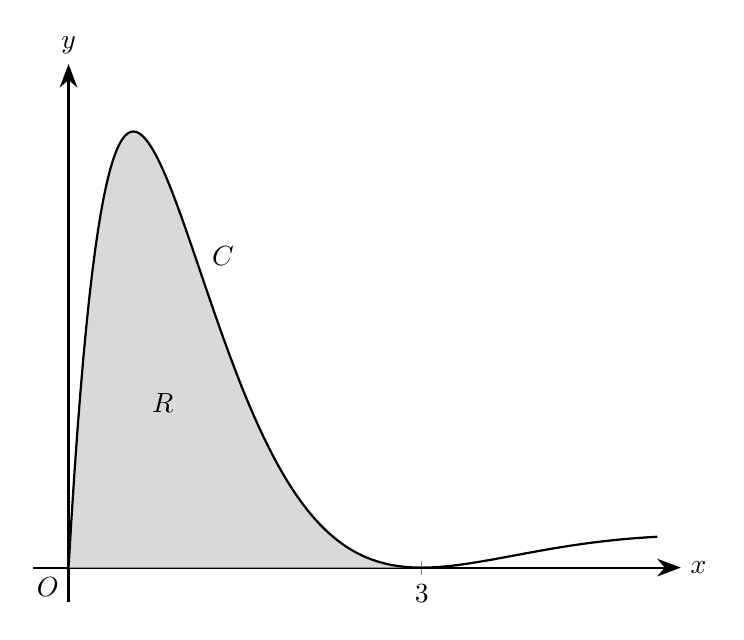
\begin{tikzpicture}[scale=1.2]
\begin{axis}[
    axis lines=middle,
    axis line style={-{Stealth[length=3mm]}, thick},
    xlabel={$x$},
    ylabel={$y$},
    xmin=-0.3, xmax=5.2,
    ymin=-0.15, ymax=2.2,
    xtick={3},
    xticklabels={$3$},
    ytick=\empty,
    clip=false,
    every axis x label/.style={at={(ticklabel* cs:1)}, anchor=west},
    every axis y label/.style={at={(ticklabel* cs:1)}, anchor=south}
]
\addplot[draw=none, name path=curvefill, samples=200, domain=0:5.0] {x*(3 - x)^2*exp(-x)};
\addplot[draw=none, name path=axisfill, domain=0:5.0] {0};
\addplot[gray!30] fill between[of=curvefill and axisfill, soft clip={domain=0:3}];
\addplot[thick, black, samples=200, domain=0:5.0] {x*(3 - x)^2*exp(-x)} node[pos=0.4, above right] {$C$};
\node at (axis cs:0.8,0.72) {$R$};
\node[below left] at (axis cs:0,0) {$O$};
\end{axis}
\end{tikzpicture}
\end{figure}


The sketch shows part of the curve $C$ given by\\

\[
y = x(3-x)^2 e^{-x} \qquad x \geq 0
\] \\
The shaded region $R$ is bounded by $C$ and the $x$-axis for $0 \leq x \leq 3$. \\

Find the exact area of $R$, giving your answer in the form
\[
A + Be^{-3}
\]
where $A$ and $B$ are rational numbers. \marks{5}

\vspace*{10pt}

\begin{tcolorbox}[colback=white, colframe=scarlet, title={\textbf{Solution}}, breakable, grow to left by=6mm, grow to right by=10mm]
For \(0 \leq x \leq 3\),
\[
x \geq 0,\qquad (3-x)^2 \geq 0,\qquad e^{-x}>0
\]
so the curve lies above the \(x\)-axis, and the required area is
\[
\int_0^3 x(3-x)^2e^{-x}\, \mathrm{d}x
\]

First expand the bracket:
\begin{align*}
x(3-x)^2
&= x(9-6x+x^2) \\
&= 9x-6x^2+x^3
\end{align*}
so
\[
\text{Area}=\int_0^3 (x^3-6x^2+9x)e^{-x}\, \mathrm{d}x
\]

Now integrate by parts repeatedly, using the tabular method:

\[
\renewcommand{\arraystretch}{1.3}
\setlength{\arraycolsep}{10pt}
\begin{array}{c|l|l}
\text{Sign} & \text{D} & \text{I} \\ \hline
+ & x^3-6x^2+9x & e^{-x} \\
- & 3x^2-12x+9 & -e^{-x} \\
+ & 6x-12 & e^{-x} \\
- & 6 & -e^{-x} \\
+ & 0 & e^{-x} \\
\end{array}
\]

Reading the table diagonally gives
\begin{align*}
\int (x^3-6x^2+9x)e^{-x}\, \mathrm{d}x
&= -(x^3-6x^2+9x)e^{-x} -(3x^2-12x+9)e^{-x} \\
&\qquad -(6x-12)e^{-x} - 6e^{-x} + C \\
&= (-x^3+3x^2-3x-3)e^{-x}+C
\end{align*}

Therefore
\begin{align*}
\text{Area}
&=\left[(-x^3+3x^2-3x-3)e^{-x}\right]_0^3 \\
&= (-27+27-9-3)e^{-3} - \bigl((-3)e^0\bigr) \\
&= -12e^{-3}+3 \\
&= 3-12e^{-3}
\end{align*}

So the exact area is
\[
3-12e^{-3}
\]
which is of the form \(A+Be^{-3}\) with
\[
A=3,\qquad B=-12
\]
\end{tcolorbox}


\newpage

% ---- Question 11 ----
\questionitem

Show that\\

\[
\int_{e^{-1/2}}^1 x(\ln x)^2\,\mathrm{d}x = a + \frac{b}{e}
\]\\

where $a$ and $b$ are rational constants to be found. \marks{6}

\vspace*{10pt}

\begin{tcolorbox}[colback=white, colframe=scarlet, title={\textbf{Solution}}, breakable, grow to left by=6mm, grow to right by=10mm]
Let
\[
I=\int_{e^{-1/2}}^{1} x(\ln x)^2\,\mathrm{d}x
\]

Use the substitution
\[
u=\ln x
\]

Then
\[
x=e^u
\qquad\text{and}\qquad
\mathrm{d}x=e^u\,\mathrm{d}u
\]

So the integrand becomes
\[
x(\ln x)^2\,\mathrm{d}x=e^u\cdot u^2\cdot e^u\,\mathrm{d}u=u^2e^{2u}\,\mathrm{d}u
\]

Now change the limits.

When $x=e^{-1/2}$,
\[
u=\ln\!\left(e^{-1/2}\right)=-\frac12
\]

When $x=1$,
\[
u=\ln 1=0
\]

Hence
\[
I=\int_{-1/2}^{0} u^2e^{2u}\,\mathrm{d}u
\]

To integrate this, use integration by parts twice.

First,
\[
\int u^2e^{2u}\,\mathrm{d}u
\]

Take
\[
p=u^2,\qquad \frac{\mathrm{d}q}{\mathrm{d}u}=e^{2u}
\]

Then
\[
\frac{\mathrm{d}p}{\mathrm{d}u}=2u,
\qquad
q=\frac12 e^{2u}
\]

So
\[
\int u^2e^{2u}\,\mathrm{d}u
=
\frac12 u^2e^{2u}-\int u e^{2u}\,\mathrm{d}u
\]

Now integrate $\int u e^{2u}\,\mathrm{d}u$ by parts again.

Take
\[
p=u,\qquad \frac{\mathrm{d}q}{\mathrm{d}u}=e^{2u}
\]

Then
\[
\frac{\mathrm{d}p}{\mathrm{d}u}=1,
\qquad
q=\frac12 e^{2u}
\]

Hence
\[
\int u e^{2u}\,\mathrm{d}u
=
\frac12 ue^{2u}-\frac12\int e^{2u}\,\mathrm{d}u
=
\frac12 ue^{2u}-\frac14 e^{2u}
\]

Substituting back,
\begin{align*}
\int u^2e^{2u}\,\mathrm{d}u
&=
\frac12 u^2e^{2u}-\left(\frac12 ue^{2u}-\frac14 e^{2u}\right) \\
&=
e^{2u}\left(\frac{u^2}{2}-\frac{u}{2}+\frac14\right)
\end{align*}

Therefore
\[
I=\left[e^{2u}\left(\frac{u^2}{2}-\frac{u}{2}+\frac14\right)\right]_{-1/2}^{0}
\]

Now substitute the limits:
\begin{align*}
I
&=
e^0\left(\frac{0^2}{2}-\frac{0}{2}+\frac14\right)
-
e^{-1}\left(\frac{(-1/2)^2}{2}-\frac{-1/2}{2}+\frac14\right) \\
&=
\frac14-\frac1e\left(\frac18+\frac14+\frac14\right) \\
&=
\frac14-\frac1e\left(\frac58\right) \\
&=
\frac14-\frac{5}{8e}
\end{align*}

So
\[
\int_{1/\sqrt e}^{1} x(\ln x)^2\,\mathrm{d}x=\frac14-\frac{5}{8e}
\]

Hence it is of the form $a+\dfrac{b}{e}$ with
\[
a=\frac14,
\qquad
b=-\frac58
\]
\end{tcolorbox}


\newpage

% ---- Question 12 ----
\questionitem

\begin{enumerate}[label=\textbf{(\alph*)}]
  \item Using the logarithmic form of $\operatorname{artanh} x$, prove that the derivative of $\operatorname{artanh} x$ is
  \[
  \frac{1}{1-x^2}
  \]
  for $|x|<1$. \marks{5} \\
  \item Hence find
  \[
  \int_0^{1/2} \operatorname{artanh} x\,\mathrm{d}x
  \]
  giving your answer in exact logarithmic form. \marks{5} \\
  \item Priya tries to evaluate
  \[
  \int_0^{3/2} \operatorname{artanh} x\,\mathrm{d}x
  \]
  using her calculator, and gets an `error'. Explain why. \marks{1} \\
\end{enumerate}

\vspace*{10pt}

\begin{tcolorbox}[colback=white, colframe=scarlet, title={\textbf{Solution}}, breakable, grow to left by=6mm, grow to right by=10mm]
\begin{enumerate}[label=\textbf{(\alph*)}]
  \item For \(|x|<1\),
\[
\operatorname{artanh} x=\frac12\ln\left(\frac{1+x}{1-x}\right)=\frac12\bigl[\ln(1+x)-\ln(1-x)\bigr]
\]
This is valid for \(|x|<1\) because we need \(1+x>0\) and \(1-x>0\).

Differentiate term by term:
\begin{align*}
\frac{\mathrm{d}}{\mathrm{d}x}\bigl(\operatorname{artanh} x\bigr)
&=\frac12\left[\frac{\mathrm{d}}{\mathrm{d}x}\ln(1+x)-\frac{\mathrm{d}}{\mathrm{d}x}\ln(1-x)\right] \\
&=\frac12\left[\frac{1}{1+x}-\frac{1}{1-x}(-1)\right] \\
&=\frac12\left[\frac{1}{1+x}+\frac{1}{1-x}\right] \\
&=\frac12\left[\frac{(1-x)+(1+x)}{(1+x)(1-x)}\right] \\
&=\frac12\left[\frac{2}{1-x^2}\right] \\
&=\frac{1}{1-x^2}
\end{align*}
Hence
\[
\frac{\mathrm{d}}{\mathrm{d}x}\bigl(\operatorname{artanh} x\bigr)=\frac{1}{1-x^2}\qquad (|x|<1)
\]

  \item Using integration by parts with
\[
u=\operatorname{artanh} x,\qquad \frac{\mathrm{d}v}{\mathrm{d}x}=1
\]
we have
\[
\frac{\mathrm{d}u}{\mathrm{d}x}=\frac{1}{1-x^2},\qquad v=x
\]
So
\begin{align*}
\int \operatorname{artanh} x\,\mathrm{d}x
&=x\operatorname{artanh} x-\int x\cdot \frac{1}{1-x^2}\,\mathrm{d}x \\
&=x\operatorname{artanh} x-\int \frac{x}{1-x^2}\,\mathrm{d}x
\end{align*}

Now let \(t=1-x^2\), so
\[
\frac{\mathrm{d}t}{\mathrm{d}x}=-2x \qquad \Rightarrow \qquad \mathrm{d}t=-2x\,\mathrm{d}x
\]
Then
\begin{align*}
\int \frac{x}{1-x^2}\,\mathrm{d}x
&=-\frac12\int \frac{1}{t}\,\mathrm{d}t \\
&=-\frac12\ln t + C \\
&=-\frac12\ln(1-x^2)+C
\end{align*}
Therefore
\[
\int \operatorname{artanh} x\,\mathrm{d}x
=x\operatorname{artanh} x+\frac12\ln(1-x^2)+C
\]

Hence
\begin{align*}
\int_0^{1/2}\operatorname{artanh} x\,\mathrm{d}x
&=\left[x\operatorname{artanh} x+\frac12\ln(1-x^2)\right]_0^{1/2} \\
&=\frac12\operatorname{artanh}\left(\frac12\right)+\frac12\ln\left(\frac34\right)-\left(0+\frac12\ln 1\right)
\end{align*}

Now
\[
\operatorname{artanh}\left(\frac12\right)=\frac12\ln\left(\frac{1+\frac12}{1-\frac12}\right)=\frac12\ln 3
\]
So
\begin{align*}
\int_0^{1/2}\operatorname{artanh} x\,\mathrm{d}x
&=\frac12\cdot \frac12\ln 3+\frac12\ln\left(\frac34\right) \\
&=\frac14\ln 3+\frac12(\ln 3-\ln 4) \\
&=\frac14\ln 3+\frac12\ln 3-\ln 2 \\
&=\frac34\ln 3-\ln 2
\end{align*}
Also,
\[
\frac34\ln 3-\ln 2=\frac14\ln\left(\frac{27}{16}\right)
\]
Therefore
\[
\int_0^{1/2}\operatorname{artanh} x\,\mathrm{d}x=\frac34\ln 3-\ln 2=\frac14\ln\left(\frac{27}{16}\right)
\]

  \item In the real number system, \(\operatorname{artanh} x\) is defined only for \(|x|<1\). The interval \([0,\tfrac32]\) includes \(x=1\), where \(\operatorname{artanh} x\) is undefined, and values \(x>1\), where it is not real. So the calculator gives a domain error.
\end{enumerate}
\end{tcolorbox}


\newpage

% ---- Question 13 ----
\questionitem

Given that
\[
y = \arcsin\left(\frac{x-1}{3}\right)
\] \\
\begin{enumerate}[label=\textbf{(\alph*)}]
  \item find $\dfrac{\mathrm{d}y}{\mathrm{d}x}$, giving your answer in its simplest form. \marks{2} \\
  \item Use integration by parts to find
  \[
  \int \arcsin\left(\frac{x-1}{3}\right)\,\mathrm{d}x
  \]
  \marks[-20pt]{4}
\end{enumerate}

\vspace*{10pt}

\begin{tcolorbox}[colback=white, colframe=scarlet, title={\textbf{Solution}}, breakable, grow to left by=6mm, grow to right by=10mm]
\begin{enumerate}[label=\textbf{(\alph*)}]
  \item Let
\[
u=\frac{x-1}{3}
\]
Then
\[
y=\arcsin u
\]
so by the chain rule,
\begin{align*}
\frac{\mathrm{d}y}{\mathrm{d}x}
&=\frac{1}{\sqrt{1-u^2}}\cdot \frac{\mathrm{d}u}{\mathrm{d}x} \\
&=\frac{1}{\sqrt{1-\left(\frac{x-1}{3}\right)^2}}\cdot \frac13 \\
&=\frac{1}{3\sqrt{1-\frac{(x-1)^2}{9}}} \\
&=\frac{1}{\sqrt{9-(x-1)^2}}
\end{align*}
Hence
\[
\frac{\mathrm{d}y}{\mathrm{d}x}=\frac{1}{\sqrt{9-(x-1)^2}}
\]

  \item Let
\[
I=\int \arcsin\left(\frac{x-1}{3}\right)\,\mathrm{d}x
\]

Use integration by parts with
\[
u=\arcsin\left(\frac{x-1}{3}\right), \qquad \frac{\mathrm{d}v}{\mathrm{d}x}=1
\]
Then
\[
v=x
\]
and from part (a),
\[
\frac{\mathrm{d}u}{\mathrm{d}x}=\frac{1}{\sqrt{9-(x-1)^2}}
\]

So
\begin{align*}
I
&=uv-\int v\,\frac{\mathrm{d}u}{\mathrm{d}x}\,\mathrm{d}x \\
&=x\arcsin\left(\frac{x-1}{3}\right)-\int \frac{x}{\sqrt{9-(x-1)^2}}\,\mathrm{d}x
\end{align*}

Now write
\[
x=(x-1)+1
\]
so
\begin{align*}
\int \frac{x}{\sqrt{9-(x-1)^2}}\,\mathrm{d}x
&=\int \frac{x-1}{\sqrt{9-(x-1)^2}}\,\mathrm{d}x+\int \frac{1}{\sqrt{9-(x-1)^2}}\,\mathrm{d}x
\end{align*}

For the first integral, let
\[
t=9-(x-1)^2
\]
Then
\[
\frac{\mathrm{d}t}{\mathrm{d}x}=-2(x-1)
\qquad \Rightarrow \qquad
(x-1)\,\mathrm{d}x=-\frac12\,\mathrm{d}t
\]
Hence
\begin{align*}
\int \frac{x-1}{\sqrt{9-(x-1)^2}}\,\mathrm{d}x
&=-\frac12\int t^{-1/2}\,\mathrm{d}t \\
&=-t^{1/2} \\
&=-\sqrt{9-(x-1)^2}
\end{align*}

For the second integral, using the result from part (a) in reverse,
\[
\int \frac{1}{\sqrt{9-(x-1)^2}}\,\mathrm{d}x
=\arcsin\left(\frac{x-1}{3}\right)
\]

Therefore
\begin{align*}
I
&=x\arcsin\left(\frac{x-1}{3}\right)-\left(-\sqrt{9-(x-1)^2}+\arcsin\left(\frac{x-1}{3}\right)\right)+C \\
&=x\arcsin\left(\frac{x-1}{3}\right)+\sqrt{9-(x-1)^2}-\arcsin\left(\frac{x-1}{3}\right)+C \\
&=(x-1)\arcsin\left(\frac{x-1}{3}\right)+\sqrt{9-(x-1)^2}+C
\end{align*}

Hence
\[
\int \arcsin\left(\frac{x-1}{3}\right)\,\mathrm{d}x
=(x-1)\arcsin\left(\frac{x-1}{3}\right)+\sqrt{9-(x-1)^2}+C
\]
\end{enumerate}
\end{tcolorbox}


\newpage

% ---- Question 14 ----
\questionitem

Use integration by parts to find
\[
\int_1^9 \sqrt{x}\ln\left(\frac{9}{x}\right)\,\mathrm{d}x
\]
giving your answer in the form $a + b\ln 3$, where $a$ and $b$ are constants to be found. \marks{5}

\vspace*{10pt}

\begin{tcolorbox}[colback=white, colframe=scarlet, title={\textbf{Solution}}, breakable, grow to left by=6mm, grow to right by=10mm]
 Let
\[
u=\ln\left(\frac{9}{x}\right), \qquad \frac{\mathrm{d}v}{\mathrm{d}x}=\sqrt{x}
\]
Then
\[
\frac{\mathrm{d}u}{\mathrm{d}x}=-\frac{1}{x}, \qquad v=\int x^{1/2}\,\mathrm{d}x=\frac{2}{3}x^{3/2}
\]

Using integration by parts,
\[
\int u\,\frac{\mathrm{d}v}{\mathrm{d}x}\,\mathrm{d}x=uv-\int v\,\frac{\mathrm{d}u}{\mathrm{d}x}\,\mathrm{d}x
\]

So if
\[
I=\int_1^9 \sqrt{x}\ln\left(\frac{9}{x}\right)\,\mathrm{d}x
\]
then
\begin{align*}
I&=\left[\frac{2}{3}x^{3/2}\ln\left(\frac{9}{x}\right)\right]_1^9
-\int_1^9 \frac{2}{3}x^{3/2}\left(-\frac{1}{x}\right)\,\mathrm{d}x\\
&=\left[\frac{2}{3}x^{3/2}\ln\left(\frac{9}{x}\right)\right]_1^9
+\frac{2}{3}\int_1^9 x^{1/2}\,\mathrm{d}x
\end{align*}

Now evaluate the first term:
\begin{align*}
\left[\frac{2}{3}x^{3/2}\ln\left(\frac{9}{x}\right)\right]_1^9
&=\frac{2}{3}(9)^{3/2}\ln\left(\frac{9}{9}\right)-\frac{2}{3}(1)^{3/2}\ln\left(\frac{9}{1}\right)\\
&=\frac{2}{3}(27)\ln 1-\frac{2}{3}\ln 9\\
&=0-\frac{2}{3}(2\ln 3)\\
&=-\frac{4}{3}\ln 3
\end{align*}

Now evaluate the integral:
\begin{align*}
\frac{2}{3}\int_1^9 x^{1/2}\,\mathrm{d}x
&=\frac{2}{3}\left[\frac{2}{3}x^{3/2}\right]_1^9\\
&=\frac{4}{9}\left((9)^{3/2}-1^{3/2}\right)\\
&=\frac{4}{9}(27-1)\\
&=\frac{104}{9}
\end{align*}

Hence
\[
I=\frac{104}{9}-\frac{4}{3}\ln 3
\]

So in the form $a+b\ln 3$,
\[
a=\frac{104}{9}, \qquad b=-\frac{4}{3}
\]
\end{tcolorbox}


\newpage

% ---- Question 15 ----
\questionitem

\[
g(\theta)=(1+\sin\theta-\cos\theta)^2
\] \\
\begin{enumerate}[label=\textbf{(\alph*)}]
  \item Show that $g(\theta)=2+2\sin\theta-2\cos\theta-\sin 2\theta$. \marks{4} \\
  \item Hence, using calculus, find the exact value of
  \[
  \int_{0}^{\frac{\pi}{2}} \theta g(\theta)\,\mathrm{d}\theta
  \]
  \marks[-30pt]{7}
\end{enumerate}

\vspace*{10pt}

\begin{tcolorbox}[colback=white, colframe=scarlet, title={\textbf{Solution}}, breakable, grow to left by=6mm, grow to right by=10mm]
\begin{enumerate}[label=\textbf{(\alph*)}]
  \item Expanding the square gives
\begin{align*}
g(\theta)
&=(1+\sin\theta-\cos\theta)^2 \\
&=1+\sin^2\theta+\cos^2\theta+2\sin\theta-2\cos\theta-2\sin\theta\cos\theta
\end{align*}

Using \(\sin^2\theta+\cos^2\theta=1\) and \(\sin 2\theta=2\sin\theta\cos\theta\),
\begin{align*}
g(\theta)
&=1+1+2\sin\theta-2\cos\theta-2\sin\theta\cos\theta \\
&=2+2\sin\theta-2\cos\theta-\sin 2\theta
\end{align*}

Hence
\[
g(\theta)=2+2\sin\theta-2\cos\theta-\sin 2\theta
\]

  \item Let
\[
I=\int_{0}^{\pi/2}\theta g(\theta)\,\mathrm{d}\theta
\]

Using part (a),
\begin{align*}
I
&=\int_{0}^{\pi/2}\theta\left(2+2\sin\theta-2\cos\theta-\sin 2\theta\right)\,\mathrm{d}\theta \\
&=2\int_{0}^{\pi/2}\theta\,\mathrm{d}\theta
+2\int_{0}^{\pi/2}\theta\sin\theta\,\mathrm{d}\theta
-2\int_{0}^{\pi/2}\theta\cos\theta\,\mathrm{d}\theta
-\int_{0}^{\pi/2}\theta\sin 2\theta\,\mathrm{d}\theta
\end{align*}

Now evaluate each integral.

First,
\begin{align*}
2\int_{0}^{\pi/2}\theta\,\mathrm{d}\theta
&=2\left[\frac{\theta^2}{2}\right]_{0}^{\pi/2} \\
&=\left[\theta^2\right]_{0}^{\pi/2} \\
&=\frac{\pi^2}{4}
\end{align*}

Next, for \(\int_{0}^{\pi/2}\theta\sin\theta\,\mathrm{d}\theta\), use integration by parts with
\(u=\theta\), \(\frac{\mathrm{d}v}{\mathrm{d}\theta}=\sin\theta\)

Then \(\frac{\mathrm{d}u}{\mathrm{d}\theta}=1\) and \(v=-\cos\theta\), so
\begin{align*}
\int_{0}^{\pi/2}\theta\sin\theta\,\mathrm{d}\theta
&=\left[-\theta\cos\theta\right]_{0}^{\pi/2}
+\int_{0}^{\pi/2}\cos\theta\,\mathrm{d}\theta \\
&=\left[-\theta\cos\theta+\sin\theta\right]_{0}^{\pi/2} \\
&=1
\end{align*}

For \(\int_{0}^{\pi/2}\theta\cos\theta\,\mathrm{d}\theta\), again use integration by parts with
\(u=\theta\), \(\frac{\mathrm{d}v}{\mathrm{d}\theta}=\cos\theta\)

Then \(\frac{\mathrm{d}u}{\mathrm{d}\theta}=1\) and \(v=\sin\theta\), so
\begin{align*}
\int_{0}^{\pi/2}\theta\cos\theta\,\mathrm{d}\theta
&=\left[\theta\sin\theta\right]_{0}^{\pi/2}
-\int_{0}^{\pi/2}\sin\theta\,\mathrm{d}\theta \\
&=\left[\theta\sin\theta+\cos\theta\right]_{0}^{\pi/2} \\
&=\frac{\pi}{2}-1
\end{align*}

For \(\int_{0}^{\pi/2}\theta\sin 2\theta\,\mathrm{d}\theta\), use integration by parts with
\(u=\theta\), \(\frac{\mathrm{d}v}{\mathrm{d}\theta}=\sin 2\theta\)

Then \(\frac{\mathrm{d}u}{\mathrm{d}\theta}=1\) and \(v=-\frac12\cos 2\theta\), so
\begin{align*}
\int_{0}^{\pi/2}\theta\sin 2\theta\,\mathrm{d}\theta
&=\left[-\frac12\theta\cos 2\theta\right]_{0}^{\pi/2}
+\frac12\int_{0}^{\pi/2}\cos 2\theta\,\mathrm{d}\theta \\
&=\left[-\frac12\theta\cos 2\theta+\frac14\sin 2\theta\right]_{0}^{\pi/2} \\
&=\frac{\pi}{4}
\end{align*}

Substituting these into \(I\),
\begin{align*}
I
&=\frac{\pi^2}{4}+2(1)-2\left(\frac{\pi}{2}-1\right)-\frac{\pi}{4} \\
&=\frac{\pi^2}{4}+2-\pi+2-\frac{\pi}{4} \\
&=\frac{\pi^2}{4}-\frac{5\pi}{4}+4 \\
&=\frac{\pi^2-5\pi+16}{4}
\end{align*}

Therefore,
\[
\int_{0}^{\pi/2}\theta g(\theta)\,\mathrm{d}\theta=\frac{\pi^2-5\pi+16}{4}
\]
\end{enumerate}
\end{tcolorbox}


\end{enumerate}
\end{document}
